
%%%%%%%%%%%%%%%%%%%%%%%%%%%%%%%%%%%%%%%%%%%%%%%%%%%%%%%%%%%%%%%%%%%%%%%%%%%%%%%%%%%%%%%%%%%%
%%%%%%%%%%%%%%%%%%%%%%%%%%%%%%%%%%%%%%%%%%%%%%%%%%%%%%%%%%%%%%%%%%%%%%%%%%%%%%%%%%%%%%%%%%%%
%%%%%%%%%%%%%%%%%%%%%%%%%%%%%%%%%%%%%%%%%%%%%%%%%%%%%%%%%%%%%%%%%%%%%%%%%%%%%%%%%%%%%%%%%%%%
%%%%%%%%%%%%%%%%%%%%%%%%%%%%%%%%%%%%%%%%%%%%%%%%%%%%%%%%%%%%%%%%%%%%%%%%%%%%%%%%%%%%%%%%%%%%
%%%%%%%%%%%%%%%%%%%%%%%%%%%%%%%%%%%%%%%%%%%%%%%%%%%%%%%%%%%%%%%%%%%%%%%%%%%%%%%%%%%%%%%%%%%%
%%%%%%%%%%%%%%%%%%%%%%%%%%%%%%%%%%%%%%%%%%%%%%%%%%%%%%%%%%%%%%%%%%%%%%%%%%%%%%%%%%%%%%%%%%%%
%%%%%%%%%%%%%%%%%%%%%%%%%%%%%%%%%%%%%%%%%%%%%%%%%%%%%%%%%%%%%%%%%%%%%%%%%%%%%%%%%%%%%%%%%%%%
%%%%%%%%%%%%%%%%%%%%%%%%%%%%%%%%%%%%%%%%%%%%%%%%%%%%%%%%%%%%%%%%%%%%%%%%%%%%%%%%%%%%%%%%%%%%
%%%%%%%%%%%%%%%%%%%%%%%%%%%%%%%%%%%%%%%%%%%%%%%%%%%%%%%%%%%%%%%%%%%%%%%%%%%%%%%%%%%%%%%%%%%%
%%%%%%%%%%%%%%%%%%%%%%%%%%%%%%%%%%%%%%%%%%%%%%%%%%%%%%%%%%%%%%%%%%%%%%%%%%%%%%%%%%%%%%%%%%%%
%%%%%%%%%%%%%%%%%%%%%%%%%%%%%%%%%%%%%%%%%%%%%%%%%%%%%%%%%%%%%%%%%%%%%%%%%%%%%%%%%%%%%%%%%%%%
%%%%%%%%%%%%%%%%%%%%%%%%%%%%%%%%%%%%%%%%%%%%%%%%%%%%%%%%%%%%%%%%%%%%%%%%%%%%%%%%%%%%%%%%%%%%



%%%%%%%%%%%%%%%%%%%%%%%%%%%%%%%%%%%%%%%%%%%%%%%%%%%%%%%%%%%%%%%%%%%%%%%%%%%%%%%%%%%%%%%%%%%%
%%%%%%%%%%%%%%%%%%%%%%%%%%%%%%%%%%%%%%%%%%%%%%%%%%%%%%%%%%%%%%%%%%%%%%%%%%%%%%%%%%%%%%%%%%%%
%%%%%%%%%%%%%%%%%%%%%%%%%%%%%%%%%%%%%%%%%%%%%%%%%%%%%%%%%%%%%%%%%%%%%%%%%%%%%%%%%%%%%%%%%%%%
%%%%%%%%%%%%%%%%%%%%%%%%%%%%%%%%%%%%%%%%%%%%%%%%%%%%%%%%%%%%%%%%%%%%%%%%%%%%%%%%%%%%%%%%%%%%
%%%%%%%%%%%%%%%%%%%%%%%%%%%%%%%%%%%%%%%%%%%%%%%%%%%%%%%%%%%%%%%%%%%%%%%%%%%%%%%%%%%%%%%%%%%%
%%%%%%%%%%%%%%%%%%%%%%%%%%%%%%%%%%%%%%%%%%%%%%%%%%%%%%%%%%%%%%%%%%%%%%%%%%%%%%%%%%%%%%%%%%%%
%%%%%%%%%%%%%%%%%%%%%%%%%%%%%%%%%%%%%%%%%%%%%%%%%%%%%%%%%%%%%%%%%%%%%%%%%%%%%%%%%%%%%%%%%%%%
\chapter{Background}\label{chap:background}
\section{Markov Decision Process}

Bellman\cite{bellamn1957mdp} in 1957 describes a framework for solving stochastic control problems. A classic example of this is playing blackjack. There is often no certain outcome to playing a given hand. However, actions exist for which the expected probability of a player winning is higher. The Markov Decision Process formalism allows one to tackle such problems systematically, with mathematically tractable convergence bounds to optimal solutions in some cases.

The MDP describes these processes as an agent acting in an environment that is, in general, partially observable.

This is described by a tuple $(\mathcal{S}, \mathcal{A}, \mathcal{R}, P, \gamma)$. $\mathcal{S}$ is the state space, the state of the world that the agent knows about, and $\mathcal{A}$ is the action space, the possible actions it may take. For a given state and action, the reward provided is real-valued and may be stochastic, $\mathcal{R}: \mathcal{S} \times \mathcal{A} \rightarrow \mathbb{R}$. $P$ are the transition probabilities between states $P: \mathcal{S} \times \mathcal{A} \times \mathcal{S} \rightarrow [0, 1]$, this defines the dynamics of the process. $\gamma $ determines the reward discount and how myopic the MDP is.

The agent aims to maximise its expected discounted cumulative reward, the return, $ \mathbb{E} [ G_t = \sum_t^T \gamma^t R_t ] $. The problem may be that of an episodic setting with a clear termination, a chess player winning, for example. Alternatively, it may be in a continuous setting with no clear termination, like managing stocks. To make decisions, an agent follows a policy. The policy, $\pi(a|s), \pi: \mathcal{S} \times \mathcal{A} \rightarrow [0, 1]$ maps states' actions to probabilities of taking action $a$, in the deterministic case it is just a map from state to action space.


A family of algorithms known as dynamic programming exists that, given finite states and actions, can find exact solutions to these problems, under reasonable constraints. However, these algorithms are often intractable for large state and action spaces.

Solutions to MDPs can be expressed in terms of the value function, $V(s) = \mathbb{E} [ G_t | s_t = s]$, which is the expected return from a given state.

The optimal value function, $V^*(s)$, is the maximum value function over all possible policies. The optimal policy, $\pi^*(s)$, is the policy that maximises the value function for all states. The optimal value function and policy satisfy the Bellman optimality equations\cite{bellamn1957mdp}:
\begin{equation}
	V^*(s) = \max_a \mathbb{E} [ R_{t+1} + \gamma V^*(s_{t+1}) | s_t = s, a_t = a].
\end{equation}

The value function is very closely linked to the action-value function $Q(s, a) = \mathbb{E} [G_t | s_t=s, a_t,=a]$ which is the expected return from taking action $a$ in state $s$ and then following the current policy, there also exists a bellman optimality equation for the action-value function:
\begin{equation}
	Q^*(s,a) = \mathbb{E} [ R_{t+1} + \gamma \max_{a'} Q^*(s_{t+1}, a') | s_t = s, a_t = a].
\end{equation}

Using dynamic programming and finding exact solutions to an MDP and the optimal policy $\pi*$ to optimise your return is often impossible. Reinforcement learning is a common alternative to dynamic programming, which provides a principled approach to learning approximate solutions. It describes a family of techniques that learn from previous experience to improve at solving MDPs.

\section{Reinforcement Learning}
Reinforcement Learning (RL) encompasses the techniques used to solve MDPs where experience is required to solve the MDP. When framed as MDPs, many real-world problems have such large state or action spaces that some approximations must be made to find any solutions. Despite the approximate nature of their solutions, RL agents have achieved superhuman performance in chess, go, starcraft and other games and have recently found diamonds in Minecraft~\cite{silver2016mastering,silver2017mastering,hafner2023mastering}. Many of these successes with current RL approaches highlight the challenges current algorithms face due to their hunger for data. Games, especially games that can be played on computers, are relatively cheap to sample data from and can be played many times\footnote{It is worth noting that RL has not just solved problems that pertain to games, but has been very successful in solving robotic control problems}. This sample hunger, combined with an inability to transfer knowledge between tasks, highlights that there is a significant advantage to encoding prior knowledge into RL algorithms. The knowledge of symmetries enables agents to attempt simplified problems and draws abstract connections between different tasks. This thesis focuses on the encoding of symmetries into RL algorithms. This section will describe the most common approaches to solving RL problems.

\section{Deep Reinforcement Learning Approaches}
The underlying optimisation problem in reinforcement learning is finding a policy which produces the maximum expected reward. However, not all RL algorithms take this approach directly. Additionally, many algorithms choose to forgo learning the dynamics of a process and instead model the value function or policy directly. These are Model-Free algorithms. In contrast, model-based algorithms learn the problem's dynamics and simulate the agent's behaviour to learn. This section will describe the most common approaches to solving RL problems.
Typically, learning algorithms face a few persistent problems in Deep RL that make solving problems difficult. These are;
\begin{itemize}
	\item \textbf{Sample Efficiency} The algorithms require a large amount of data to learn. This is because training large neural networks requires lots of data to learn. As mentioned before, breakthroughs in RL are often made in games, where data can be simulated and collected cheaply\cite{dulac2019challenges}
	\item \textbf{Training Robustness} The algorithms can often struggle to converge depending on the initialisation of the environment and the agent, and special random seeds are required to see good performance\cite{henderson2018deep}.
	\item \textbf{Reward Sparsity} Reward functions are often sparse, and coming across states that provide rewards, such as finding diamonds in Minecraft, is a difficult problem when initial exploration is random.\cite{hafner2023mastering}.
\end{itemize}

\subsection{Model Based Algorithms}
Model-based reinforcement learning is the process of the agent learning the dynamics of a system and then performing "planning" to decide how best to act next. In concrete terms, this corresponds to an agent learning the transition dynamics of the MDP, thus learning both the subsequent state of a state action pair, $P(s'| s, a)$ and the expected reward from a state action pair $r(s, a)$. From the learned model agent "plans" by simulating the environment and acting in the simulated environment. Then the agent learns a policy with the simulated data. Common algorithms like Dyna-Q, use Q-learning over a comnination of real and simulated data to learn a policy.

Model-based algorithms have the potential to provide much better sample efficiency than model-free algorithms, as they can learn from simulated data. However, this in itself can be difficult to learn. However, the Dreamer models have shown substantial success in tackling difficult problems\cite{hafner2023mastering, hafner2020mastering}. This report does in some way, build a world model.
....NEEDS MORE..... I could do with actually knowing more about this and having build some model free instances to figure out this
\subsection{Model Free Algorithms}
Model-free algorithms forgo trying to build an approximation of the MDP's transition dynamics defined by $P$ and instead try to optimise the agent behaviour by either approximating how good different states are or learning the best action to take in given states. When combining standard dynamic programming algorithms such as q-learning with function approximation, or actor-critic methods, the challenge is finding a way to learn the form of the parametric function approximator, which is often a neural network. As such, there is a common approach between multiple algorithms, where you form a supervised learning problem, finding a function that minimises a loss. In the RL setting, the data is gained from the MDP. The fundamental difference between Q-Learning and Actor-Critic approaches is that Q-learning uses an epsilon greedy policy to collect data and experience. Whereas, Actor Critics learn a stochastic policy from the data. However, the training loop is much the same;
\begin{algorithm}
	\caption{Model Free RL Training Loop}
	\begin{algorithmic}
		\State Initialise $\theta$ randomly.
		\Comment{Network Parameters}
		\State Initialise $t=0$
		\Comment{Buffer Timestep}
		\State Initialise $T=0$
		\Comment{Total Timestep}
		\State Initialise replay buffer $\mathcal{D} \leftarrow \emptyset$
		\State Sample state $s$
		\While $\text{ }T < T_{max}$
		\State Take action $a$ according to policy $\pi(a|s)$
		\State Observe reward $r$ and next state $s'$
		\State Store transition $(s, a, r)$ in replay buffer $\mathcal{D}$
		\LComment {Replay buffer respects temporal order of experience.}
		\State $s \leftarrow s'$
		\State $t \leftarrow t+1$
		\State $T \leftarrow T+1$
		\LComment{If a state is terminal, then reset the environment. Continue to sample experience. Masking is used to ensure that terminal states have zero value.}
		\If{$t \mod T_{experience} == 0$}
		\Comment{ Update Loop}
		\State Perform minibatch gradient descent updates $\theta$ to minimise $L(\mathcal{D},\theta)$
		\LComment{Where $L$ is the loss function, these losses are very different in the AC and Q-Learning, but the training loop is the same.}
		\State $t \leftarrow 0$
		\State $\mathcal{D} \leftarrow \emptyset$
		\EndIf

		\EndWhile

	\end{algorithmic}
\end{algorithm}
In most cases, some operations need to be performed on the replay buffer, and the buffer will store more data than just sequential $(s, a,r)_t$ tuples. Often subsequent actions are required to calculate the loss. This can be done during the update loop. Finally, rather than interacting with one environment, training is done in parallel in multiple environments. The process is much the same; states, rewards and actions become vectors for this. Environment vectorisation has improved training stability and robustness~\cite{minh2016asynchronous}.

\subsubsection{Deep Q-Learning}
Q-Learning forgoes optimising the true objective, the policy, to learn the optimal value function. This allows one to find an optimal policy, as there is always a greedy policy with a stationary point at the optimal value function. Dynamic Programming exploits this idea in algorithms such as Value Iteration\cite{bellamn1957mdp} and Policy Iteration\cite{howard1960dynamic}.

When extended to function approximation the convergence guarantees of the origianl dynmaic programming Q-learning algroithm are absent in Deep-Q-Learning. While exact solution may not be found due to computational restraints or partial observability, excellent solutions can be found in practice using this method~\cite{mnih2013playing}. Traditional Q learning updates the value of the current state-action pair, $Q(s, a)$, using the Bellman optimality equation for the action-value function,
\begin{equation}
	Q_{t+1}(s, a) = Q_t(s,a) + \alpha \left[ r(s, a) + \gamma \max_{a'} Q_t(S_{t+1}, a') \right].
\end{equation}
Where $\alpha$ is the step size, all other symbols take their normal values. The important point is that this converges to the optimal value function given infinite state action space visitation. In the setting of Deep Q Learning, we lose the guarantees of convergence in exchange for flexibility.

The Bellman optimality equation can be used to construct a loss function to train a parametric function approximation, a deep learning model, through gradient methods, If this method were employed in an on-policy fashion with a deterministic greedy optimal policy, there would be no exploration. As such, the agent would not gain new experience, so an alternative exploration policy is used. The results of its trajectory or trajectories, depending on whether it is an episodic setting, are stored in a Replay Buffer,
\begin{equation}
	\mathcal{D} = \{S_0, A_0, R_1, S_1, A_1, \ldots \}
\end{equation}
This can be sampled when training the network. The loss function to optimise is derived from the Bellman equation and is the squared temoporal difference error\cite{sutton2018reinforcement},
\begin{equation}
	L_{w}(\mathcal{D}) = \mathbb{E}_{(s,a,r,s') \sim \mathcal{D}}\left[\left(Q_w(s,a) -(r + \gamma(1-\mathbb{I}(s'= S_{T}))\max_{a'}Q_{w'}(s', a')\right)^2\right].
\end{equation}
Here, it is essential to note that $Q_w'$ can be the original network if $w = w'$. However, there are some problems associated with this. The gradient with respect to the loss must now become a semi-gradient, to allow the bootstrapping off one's own predictions, where the $Q_w'$ term must be considered a constant with respect to $w$. The indicator, $\mathbb{I}(s' = S_T)$,  is one if $s'$ is a terminal state.

Alternatively, the semi-gradient can be avoided with Double-Q-Learning. Double-Q-Learning uses target networks\cite{van2016deep}. This makes two copies of the primary, $Q_w$, network and performs gradient updates on one, $Q_w$, with the secondary network, $Q_{w'}$, parameters being moved towards $w$ after some further number of updates so that its parameters lag that of $w$. This can be done with weighted averages or just a direct update.

Some problems arise in continuous state spaces, where the $\max$ operation may involve an optimisation loop. This is not ideal. Algorithms such as DDPG\cite{lillicrap2015continuous} use another network to parameterise an optimal policy instead of the max operation. DDPG is an example of an Actor-Critic algorithm that straddles the divide between Q-Learning and Policy Based Methods.


\subsubsection{Policy Based Methods}
While Policy Based Methods all strive to optimise the expected cumulative return for an agent, there are quite a few subtleties between the dominant gradient-based approaches. In the episodic setting, where it is possible to obtain complete trajectories and optimise for episodic returns, policy gradient functions can directly optimise the expected cumulative reward,
\begin{equation}
	J_G(\theta) = \mathbb{E}_{s_0 \sim d_0}\left[v_{\pi_{\theta}}(S_0)\right].
\end{equation}
However, in infinite time horizon tasks, there is no termination and optimising for the expected reward of the next action may be a more prudent objective,
\begin{equation}
	J_R(\theta)
	= \mathbb{E}_{\pi_{\theta}}\left[R_{t+1}\right].
\end{equation}
Many common algorithms for episodic tasks can be extended for infinite time horizon problems.
In both cases, it should be noted that the objective function from which we are taking the gradient is an expectation. This provides a problem, and we use the score function trick to take the gradient before the expectation.

It is possibel to use the score function trick to derive the gradient-based update term in the episodic case. First, the expected reward is expressed in its natural form as the average return under the distribution of trajectories defined by the policy and the MDP's dynamics and proceed to do some algebra to get it into a more friendly form,
\begin{align}
	\nabla_\theta J_G(\theta) & = \nabla_\theta \mathbb{E}_{\tau \sim \pi_\theta}\left[R(\tau)\right]                            \\
	                          & = \nabla_\theta \sum_\tau R(\tau) P(\tau|\theta)                                                 \\
	                          & = \sum_\tau R(\tau) \nabla_\theta P(\tau | \theta)                                               \\
	                          & = \sum_\tau R(\tau) P(\tau | \theta) \frac{\nabla_\theta P(\tau | \theta)}{P(\tau |\theta)}      \\
	                          & = \mathbb{E}_{\tau \sim \pi_{\theta}} \left[ R(\tau) \nabla_\theta \log(P(\tau| \theta))\right].
\end{align}
It would be ideal if the trajectories' probability could be calculated without any knowledge of the MDP's dynamics $P(S_{t+1}| S_t, A_t)$. This can be done by exploiting the definition of the trajectory's probability.
\begin{equation}
	P(\tau|\theta) = P(S_0) \prod_{t=0}^ TP(S_{t+1}| S_t, A_t)\pi_\theta(A_{t}|S_{t})
\end{equation}
Thus using log rules, the expectations can be rearranged in the form,
\begin{align}
	\nabla_\theta J_G(\theta)  = \mathbb{E}_{\tau \sim \pi_{\theta}} & \left[ R(\tau) \nabla_\theta  \right.                                                                               \\
	                                                                 & \left. \left\{ \log(P(S_0)) +  \sum_{t=0}^ T \log(P(S_{t+1}| S_t, A_t))+ \log(\pi_\theta(A_t|S_t))\right\} \right], \\
	= \mathbb{E}_{\tau \sim \pi_{\theta}}                            & \left[ R(\tau) \nabla_\theta \sum_{t=0}^ T \log(\pi_\theta(A_t|S_t))\right].
\end{align}
With this form of the policy gradient, we could sample multiple trajectories and perform gradient descent on the policy.

This would be an unbiased estimate of the policy gradient. Empirically, the variance of the gradient updates for deep networks is inefficient in the number of training samples or impossible, depending on the task. One further remedy to this is that we can note that a policy at time $t = t'$ should not depend on the rewards in the past; this insight can be seen by splitting the expectation,
\begin{align}
	\nabla_{\theta} J_G(\theta) & = \mathbb{E}_{\tau \sim \pi_{\theta}} \left[ R(\tau) \nabla_\theta \sum_{t=0}^ T \log(\pi_\theta(A_t|S_t))\right]                                               \\
	                            & = \mathbb{E}_{\tau \sim \pi_{\theta}} \left[ \left(\sum_{k = 0}^T r(S_k, A_k)\right) \left(\nabla_\theta \sum_{t=0}^ T \log(\pi_\theta(A_t|S_t))\right) \right] \\
	                            & = \sum_{t = 0} ^T \mathbb{E}_{\tau \sim \pi_\theta} \left[ \sum_{k = 0} ^ {t-1} r(S_k, A_k) \nabla_\theta \log(\pi_\theta(A_t|S_t)) \right.                     \\
	                            & \left. + \sum_{k' = t} ^ T r(S_{k'}, A_{k'}) \nabla_\theta \log(\pi_\theta(A_t| S_t)) \right ]. \label{causal_expect}
\end{align}
As the rewards at time $t$ are only correlated to the actions only at time $t$, and none of the previous times, the left-hand side of the expectation can be factorised into two expectations,
\begin{equation}
	\mathbb{E}_{\tau \sim \pi_\theta} \left[ \sum_{k = 0} ^ {t-1} r(S_k, A_k) \nabla_\theta \log(\pi_\theta(A_t|S_t))\right]
\end{equation}
\begin{align*}
	 & = \mathbb{E}_{\tau \sim \pi_\theta} \left[ \sum_{k=0}^{t-1}r(S_k, A_k)\right] \mathbb{E}_{\tau \sim \pi_\theta} \left[ \nabla_\theta \log(A_t| S_t) \right]                                                                 \\
	 & = \mathbb{E}_{\tau \sim \pi_\theta} \left[ \sum_{k=0}^{t-1}r(S_k, A_k)\right] \mathbb{E}_{\tau \sim \pi_\theta} \left[ \frac{\nabla_\theta \pi_\theta(A_t| S_t)}{\pi_\theta(A_t| S_t)} \right] \label{score_function_lemma} \\
	 & = \mathbb{E}_{\tau \sim \pi_\theta} \left[ \sum_{k=0}^{t-1}r(S_k, A_k)\right] \sum_{A_t} \pi_\theta(A_t|S_t)\frac{\nabla_\theta \pi_\theta(A_t| S_t)}{\pi_\theta(A_t| S_t)}                                                 \\
	 & = 0.
\end{align*}
Thus equation\ref{causal_expect} becomes,
\begin{align}
	 & = \sum_{t = 0} ^T \mathbb{E}_{\tau \sim \pi_\theta} \left [  \sum_{k' = t} ^T  r(S_{k'}, A_{k'}) \nabla_\theta \log(\pi_\theta(A_t| S_t)) \right ].
\end{align}
The sum over future rewards is the expected return. Combined with the log derivative's expectation of zero. This formulation enables lower variance updates with the same expectation. A detailed review of this is available in~\cite{schulman2015highdimensional}. The general policy gradient is of the form,
\begin{equation}
	\nabla J_G(\theta)  = \mathbb{E}_{\tau \sim \pi_\theta} \left[\sum_{t=0} ^ T \mathcal{R}_t \nabla_\theta \log(\pi_\theta(A_t|S_t))\right].
\end{equation}
Where $\mathcal{R}_t$ is a return estimator a time $t$, if the return estimator is the discounted sum of rewards, this is the REINFORCE algorithm~\cite{williams1992simple}.
The most used modern policy gradient algorithms take this form: a return estimator either sampled or bootstrapped with a possible constant baseline offset. This leads to Actor-Critic methods, where the actor is the policy network, and the critic is a value function estimation network.

\subsubsection{Actor Critic Methods}
Actor critics in deep learning typically consist of a pair of function approximation networks, one the actor to approximate the optimal policy, the other to approximate the optimal value function. Because the gradient of a constant is zero, having a baseline that is independent of the policy does not affect the expectation of the policy gradient estimator, but if picked wisely, it may reduce the variance,
\begin{equation}
	\nabla J_G(\theta)  = \mathbb{E}_{\tau \sim \pi_\theta} \left[\sum_{t=0} ^ T (\mathcal{R}_t - b) \nabla_\theta \log(\pi_\theta(A_t|S_t))\right].
\end{equation}
As the variance of the updates depends on the magnitude of the $(\mathcal{R}_t - b)$ term, a function is learned to estimate the value of the state, $V_\phi(S_t)$, and the baseline is set to the value of the state, $b = V_\phi(S_t)$. The critic trained to minimise the mean squared error between the estimated value and the actual return. This produces an unbiased update of lower variance, which has better training behaviour\cite{sutton2018reinforcement}.

\subsection{Generalised Advantage Estimation}
Generalised advantage estimation\cite{schulman2015high}, rather than using the discounted return as a learning target. It learns the $\lambda$-return, a weighted sum of the n-step discounted returns. The $\lambda$-return is defined as,
\begin{equation}
	R_t^\lambda = (1-\lambda) \sum_{n=1}^\infty \lambda^{n-1} R_{t:t+n}^V.
\end{equation}
Where $R_{t:t+n}^V$ is the n-step discounted return and lambda is a hyperparameter that controls the trade-off between bias and variance on the return estimator as it gradually uses its own estimates for states values, when $\lambda = 0$, it is an unbiased return estimate. The n-step discounted return is defined as,
\begin{equation}
	R_{t:t+n}^V = \sum_{k=0}^{n-1} \gamma^k r_{t+k} + \gamma^n V_\phi(S_{t+n}).
\end{equation}
The lambda return provides a biased but lower variance return estimator, which can benefit training and is the backbone of many modern policy gradient algorithms. Typically the lambda return is calculated recursively backwards in episodic settings,
\begin{equation}
	R_t^\lambda = r_t + \gamma (1-\lambda) V_\phi(S_{t+1}) + \lambda R_{t+1}^\lambda.
\end{equation}
And then the advantage is the difference between the value function and the lambda return,
\begin{equation}
	A_t^\lambda = R_t^\lambda - V_\phi(S_t).
\end{equation}
Having the generalised advantage as the optimisation target provides control over the variance of the gradient estimator. The generalised advantage estimator is defined as,
\begin{equation}
	\nabla J_G(\theta)  = \mathbb{E}_{\tau \sim \pi_\theta} \left[\sum_{t=0} ^ T A_t^\lambda \nabla_\theta \log(\pi_\theta(A_t|S_t))\right].
\end{equation}
In this situation, the critic network learns to minimise the advantage. Advantage estimation is often used with regularisation methods that stop the current policy from moving too far between training updates. These regularisation methods penalise the KL divergence between the current and previous policies. This is the case for TRPO\cite{shculman2015trust} and the computationally efficient and simple PPO\cite{schulman2017proximal}.

\subsubsection{PPO}
Proximal policy optimisation (PPO) follows the same lines as TRPO, as it is a regularised form of gradient-based policy optimisation with a critic that learns a value function as a bias reduction method. The PPO paper introduces two forms: a hard thresholding method PPO-Clip, and a soft regularisation method PPO-Penalty. The clip optimisation target removes the need for explicitly calculating a KL-divergence for a single interaction is,
\begin{equation}
	L(s, a, \theta_k, \theta) = \min \left( \frac{\pi_\theta(a|s)}{\pi_{\theta_k}(a|s)} A^{\pi_{\theta_k}}(s,a), g\left(\epsilon, \frac{\pi_\theta(a|s)}{\pi_{\theta_k}(a|s)} \right)A^{\pi_{\theta_k}}(s, a) \right).
\end{equation}
Where the update rule is defined by the gradient descent algorithm, and $\theta_k$ is the previous value of $\theta$. The advantage of a policy $\pi$ is given by a truncated $\lambda$-return,
\begin{equation}
	A^{\pi}(s, a) = V^\pi _\phi(s) - R_t(s, a).
\end{equation}
Where the $V^\pi _ \phi(s)$ is the critic, typically a neural network. $R_t(s, a)$ is the sampled return for the state action pair. As the algorithm is off-policy, there is an importance-sampling correction to the advantage. To stop wide variance in the policy, like TRPO, the magnitude of the update is capped with the $g$ function,
\begin{equation}
	g(\epsilon, A) = (1 + \text{sign}(A)\epsilon)A.
\end{equation}
The $\epsilon$ hyperparameter must be set. This loss function ensures that there are no overly large policy updates.


\section{Groups, Symmetries, Homomorphisms}

\subsection{Groups}
Groups are an abstract mathematical idea on a set with a binary operation, "$\cdot$". To form a group, the members of a set must satisfy the following:
\begin{itemize}
	\item[1] Closure: applying the group's operation maps all elements back onto another element.
	\item[2] Possession of an identity element: there must be an element of the set such that it and any element is mapped onto itself.
	\item[3] Possession of inverse elements: every element in the group has an inverse element.
	\item [4] Associativity: $(a \cdot b) \cdot c = a \cdot (b \cdot c) \text{  }\forall a, b, c$
\end{itemize}
The key point is that specific symmetries form groups of all the transformations that leave the object/space invariant.

\subsection{Representation and Actions}
Members of groups like roation operations or flip operations maintain their properties no matter what space you are in, for example flipping an image or a function the group is still the same, in that if you perform two flips you get the same image/function as such the group is a very general and abstract concept. When dealing with groups, in a concrete setting then the group is a set of matricies or functionals that operate on a space or a function, these are in general described as group actions, for our purposes only the left action is needed. The group action is defined as,
\begin{equation}
	\ell_g: \mathcal{X} \times G \rightarrow \mathcal{X}, \forall g \in G, \forall x \in \mathcal{X}.
\end{equation}
Where $\mathcal{X}$ is an arbitrary set and the left action obeys the following properties:
\begin{itemize}
	\item[1] $\ell_{g_1}(\ell_{g_2}(x)) = \ell_{g_1 \cdot g_2}(x)$.
	\item[2] $\ell_e(x) = x$.
\end{itemize}
Additionally Because of the definintion of a group action, the aplication of a group action to a function is equal to the function applied to the inverse of the group action applied to the functions domain, i.e.
\begin{equation}
	\ell_g(f(x)) = f(\ell_{g^{-1}}(x)).
\end{equation}

The inverse group action is commonly written as $\ell_{g^{-1}}(x) = g^{-1}x$, when acting on the domain of a funtion.

In the special case of vector spaces the group actions are invertable matricies and are called a representation;
\begin{equation}
	\pi_g^\mathcal{V}: G \rightarrow GL(\mathcal{V}), \forall g \in G.
\end{equation}
Where $\mathcal{V} \in \mathbb{R}^n$ is a vector space, and the group representaiton $\pi_g^\mathcal{V}$ is an invertable matrix. These representations also follow the properties of the group, i.e. they are invertable, and the identity element is mapped to the identity matrix.
\subsection{Invariances}
Invariances are properties maintained under a transformation of the input space, e.g.\ mirror symmetry, where the distance to a point on the mirror line is the same from the left and the right if the object is symmetric. If you have a function $f: \mathcal{X} \rightarrow \mathcal{Y}$ that is invariant to a transformation $\ell_g(x): \mathcal{X} \times G \rightarrow \mathcal{X}$, this is expressed as:
\begin{equation}
	f(x) = f(\ell_g(x)),   \forall g \in G, \forall x \in \mathcal{X}.
\end{equation}
For the transformation to be a group, there must also include the identity element s.t $\ell_h(x) = x,  h \in G, \forall x\in \mathcal{X}$. This is how symmetry is typically expressed. The symmetry belongs to an abstract group. For example, suppose an object has 3-fold rotation symmetry around an axis. In that case, an abstract group with operations between its elements mirrors that of rotations around the axis by $120^o, 240^o$ and $0^o$. It is straightforward to check that these operations form a group. Rotations by $360^o$ left or right are the identity element. The group is closed; no matter how many rotations are performed, the object with the symmetry is still the same. The inverse of the rotation by $120^o$ is the rotation by $240^o$ and vice versa. Finally, the rotations are associative. This is the group of symmetries of the object. The object is invariant to the transformations in the group.

\subsection{Equivariance}
Equivariance is related in that if there is some transformation $\ell_g: \mathcal{Y} \times G \rightarrow \mathcal{Y}$, where it is a different representation of the group, equivariance which is a more general statement than invariance is,
\begin{equation}
	\ell_g^\mathcal{Y}( f(x) )= f(\ell_g^\mathcal{X}( x)), \forall g \in G, \forall x \in \mathcal{X}.
\end{equation}
Here, both $\ell_g$s are actions of the same group member. However, the spaces they act upon are different. This notion is especially important in the space of RL.\ From this definition, we can see that invariance is a particular case of equivariance where $\ell^\mathcal{Y}_g$ is the identity, $\forall g \in G$.
\subsection{Homomorphisms}
A homomorphism describes a map between two structures that preserves an operation. In the context of reinforcement learning, the preservation is that of the dynamics of a Markov Decision Process.

%%%%%%%%%%%%%%%%%%%%%%%%%%%%%%%%%%%%%%%%%%%%%%%%%%%%%%%%%%%%%%%%%%%%%%%%%%%%%%%%%%%%%%%%%%%%%%
%%%%%%%%%%%%%%%%%%%%%%%%%%%%%%%%%%%%%%%%%%%%%%%%%%%%%%%%%%%%%%%%%%%%%%%%%%%%%%%%%%%%%%%%%%%%%%
\section{MDP Homomorphism}
An MDP homomorphism describes a surjective mapping between one MDP and another; Ravindran and Barto first described this notion in the early 2000s\cite{ravindran2003smdp,ravindran2001symmetries}.

\textbf{Definition: MDP Homomorphism} Given some MDP $\mathcal{M}$, where there exists a surjective map, from $\mathcal{S} \times \mathcal{A} \rightarrow \overline{\mathcal{S}} \times \overline{\mathcal{A}}$. The MDP $\overline{\mathcal{M}}$\footnote{All abstract quantities are denoted with an $\overline{\text{overline}}$} is an abstract MDP over the new space. The homomorphism $h$, then is the tuple of $(\sigma, \alpha_s|s \in \mathcal{S})$, where $\sigma: \mathcal{S} \rightarrow \overline{\mathcal{S}}$ and $\alpha_s : \mathcal{A} \rightarrow \overline{\mathcal{A}}$. This surjective map must satisfy two constraints for it to be a valid MDP homomorphism;
\begin{enumerate}
	\item $R(s, a) = R(\sigma(s), \alpha_s(a))$
	\item $P(s'| a, s) = P(\sigma(s')| \alpha_s(a), \sigma(s))$
\end{enumerate}

Given this formulation, they show that there are equivalences between the real optimal value function and the optimal abstract value function,
\begin{align*}
	V^*(s)    & = \overline{V}^*(\sigma(s)).              \\
	Q^*(s, a) & = \overline{Q}^*(\sigma(s), \alpha_s(a)).
\end{align*}
This is \textit{optimal value equivalence}. Further, they introduced the idea of "lifting", where a policy learned in the abstract space can be mapped to the original space. The lifted policy $\pi^\uparrow$ is related to the abstract policy $\overline{\pi}$ by dividing by the preimage, the set of inputs to the homomorphic mapping that map to the same output.
\begin{equation}
	\pi^\uparrow(a | s) = \frac{\overline{\pi}(\alpha_s(a) | \sigma(s))}{| a \in \alpha^{-1}_s(\bar{a})|}.
\end{equation}
As such any solution found in an abstract MDP can easily be transferred to the orginal MDP.
\subsection{Group Structured MDP Homomorphisms}
A natural homomorphic mapping is that of an MDP that possesses symmetry, which is concretised by having the homomorphisms be the representations of the group in state and action space,
\begin{enumerate}
	\item $R(s, a) = (\ell^\mathcal{S}_g(s), \ell^\mathcal{A}_g(a))$,
	\item $P(s'| a, s) =P(\ell^\mathcal{S}(s')| \ell^\mathcal{A}(a), \ell^\mathcal{S}(s))$.
\end{enumerate}
Where $\ell_g^\mathcal{X}$ is the representation of the element $g \in G$ in the space $\mathcal{X}$, in plain English, for each state or state action pair, there are a set of states with the same reward and transition probability to some new state, where these states are related to each other by the operations of the elements of g on them.



The abstract MDP can then be solved with Dynamic Programming or approximate Dynamic Programming techniques, and the policy found in the abstract MDP can be "lifted" to the original MDP.



\section{The Infamous Cartpole}
\begin{figure}[h!]
	\centering
	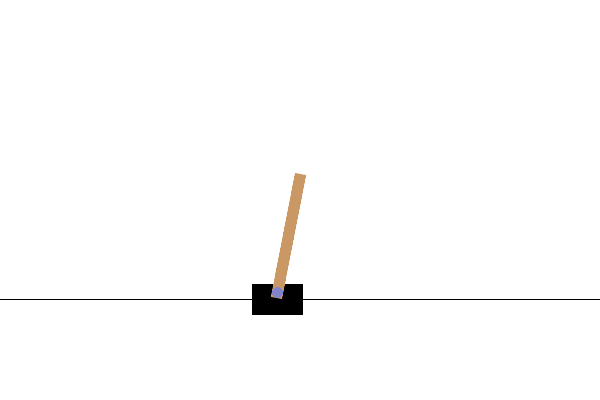
\includegraphics[width=0.5\textwidth]{Figures/cart_pole.png}
	\caption{The Cartpole environment.}
\end{figure}
The Cartpole environment is the "Hello World" of reinforcement learning; it describes a game where at each timestep, the aim is to balance a mass above a slider, 1 point is given for each timestep that the mass makes an angle of fewer than 12 degrees from vertical. The action space$a \in {0,1}$, for the problem, is to either push the pole left or right. The state space is the position of the cart, the velocity of the cart, the angle of the pole and the angular velocity of the pole; as such, $s \in \mathbb{R}^4$. Typically, the episodes are truncated at 500 timesteps, and the reward is 1, so the return is an integer $G_0 \in [0, 500]$. An episode terminates if the pole falls over or the cart moves too far from the centre. If a human were learning to solve this problem, one would notice that the expected result of pushing the cart left when it is leaning right at some positions is the same as pushing the cart right when it is leaning left at the displacement in the opposite direction. This is an example of symmetry in the problem, and it is this symmetry that we will attempt to exploit to improve the learning characteristics of the agent.

The symmetry present in Cartpole is the cyclic $C_2$ group. Other than the trivial group, the group with a single element, the $C_2$ group, is the simplest. This is a group with only two elements, the identity and inversion.
\begin{table}[h!]
	\centering
	\begin{tabular}{c | c  c}
		$C_2$ & $e$ & $r$ \\
		\hline
		$e$   & $e$ & $r$ \\
		$r$   & $r$ & $e$
	\end{tabular}
	\caption{The $C_2$ group table, where entry $i, j$ is the result of group operation on the $i^{th}$ and $j^{th}$ element.}
\end{table}


As such, to find the group structured MDP homomorphism, the agent needs to learn an equivariant mapping that respects $\pi_1^s\mathbf{s} = \mathbf{s}$ and $\pi_r^s\mathbf{s} = -\mathbf{s}$, as well as $\pi_1^a\mathbf{a} = \mathbf{a}$ and $\pi_r^a\mathbf{a} = 1 - \mathbf{a}$. Here the state and actions as vectors; $\mathbf{s}, \mathbf{a}$ are being acted upon by the vector representations of $C_2, \pi$ in their respective spaces.


\section{Neural Networks and The Inductive Biases}

What is nice in many ways about the original MLP model is that it is so flexible, however this also highlights one of its weaknesses when solving applied problems, because in theory MLPs have incredible expressive power, they are perfectly able to represent impossible functions, when applied to domains such as Images, and physical processes where there are concrete rules governing the processes that are being modelled\footnote{See the last few hundred years of Physics for examples.}. Additionally it is posited by~\cite{wolpert1995no}, that there is no free lunch in machine learning, and that there must be a constrained search space for possible algorithms. Such Constraints are in other words, inductive biases~\cite{baxter2000model}. This kind of reasoning has lead to much research into encoding inductive biases into Deep Networks, from~\cite{goyal2022inductive} a table of current approaches to introduce inductive biases;

\begin{table}
	\centering
\begin{tabular}{|c | c|}
	\hline
	Inductive Bias              & Corresponding property                              \\
	\hline
	\hline
	Distributed representations & Inputs mapped to patterns of features               \\
	\hline
	Convolution                 & group equivariance (usually over space)             \\
	\hline
	Deep architectures          & Complicated functions = composition of simpler ones \\
	\hline
	Graph Neural Networks       & equivariance over entities and relations            \\
	\hline
	Recurrent Nets              & equivariance over time                              \\
	\hline
	Soft attention              & equivariance over permutations                      \\
	\hline
	Self-supervised             & pre-training $P(X)$ is informative about $P(Y |X)$      \\
	\hline
\end{tabular}
\end{table}

For the purposes of this thesis, the focus will be on the induction of group eqivariances. However, it is important to note that this strategy to improving Machine Learning models comes from a more general class of ideas.


\subsection{Neural Networks and The Raiders of the Group}
\subsection{G-CNNs}\label{sec:G-CNNs}

The Group Equivariant Convolutional Neural Network (G-CNN) is a generalisation of the CNN's translational equivariance to arbitrary group structured equivariances.

The traditional Convolution layer is a discrete convolution, this is an approximation of tha continuous convolution,
\begin{equation}
	(f*g)(x) = \int_{\mathbb{R}^d} k(x-x')f(x')dy,
\end{equation}
where $f$ and $k$ are functions on $\mathbb{R}^d$. What can be noticed is that this is infact the definition of the cross correlaion between $f$ and $\ell_g[k]:  \mathbb{R}^d  \rightarrow \mathbb{R}^d$, where $\ell_g[k]$
is the translation group $\mathbb{R}^d$ acting on the kernel $k$,
\begin{align}
	(f*g)(x) & = \int_{\mathbb{R}^d} k(x-x')f(x')dx'       \\
	         & = \int_{\mathbb{R}^d} k(g^{-1}x')f(x')dx'   \\
	         & = \int_{\mathbb{R}^d} \ell_g[k](x')f(x')dx'
\end{align}
Here, the inverse of a tranlastion by $x$, group action $g$ is the translation by $-x$. This is then $g^{-1}$, the inverse of the group action. This is the backbone of the G-CNN\cite{cohen2016group}, where rather than a translation group, we have an arbitrary group $G$ acting on the kernel $k$. When looking for more complex equivariances than $C_2$, multiple different groups can be used in the same layer, this increases the number of varibles in the convolution's output, this complecates the form of the layers, however for our purposes this is not relevant.


\subsection{Steerabel Kernel G-CNNs}
% TODO: Add a section on Steerable Kernel G-CNNs